\documentclass[11pt,a5paper,footinclude=true,headinclude=true, oneside]{scrbook}
\usepackage[T1]{fontenc} 
\usepackage{graphicx}
\usepackage{lipsum}
\usepackage[linedheaders,parts,pdfspacing]{classicthesis} % ,manychapters
%\usepackage[osf]{libertine}
\usepackage{amsthm}
\bibliographystyle{IEEEtran}

\begin{document}

\begin{titlepage}
   \begin{center}
       \vspace*{1cm}

        \begin{figure}[htbp]
            \centerline{
\includegraphics[scale=.5]{hs-hl.jpg}}
        \end{figure}
       \textbf{Drone Application in Precision Agriculture}
            
       \vspace{0.5cm}

       \textbf{Vytaras Juraska}

       \vfill
            
       \vspace{0.8cm}
            
       Electronics Engineering student of\\
       Hamm-Lippstadt Hochschule\\
            
   \end{center}
\end{titlepage}

%	\pagestyle{scrheadings}
%	\manualmark
%	\markboth{\spacedlowsmallcaps{\contentsname}}{\spacedlowsmallcaps{\contentsname}}
	
	\tableofcontents 

%	\automark[section]{chapter}
%	\renewcommand{\chaptermark}[1]{\markboth{\spacedlowsmallcaps{#1}}{\spacedlowsmallcaps{#1}}}
%	\renewcommand{\sectionmark}[1]{\markright{\thesection\enspace\spacedlowsmallcaps{#1}}}

    % use \cleardoublepage here to avoid problems with pdfbookmark
\chapter{Introduction}
	
Over the years, a lot of burning questions come up, which deducts how well and for how long the human race can survive for on the land, that we've got. There are many, still unsolved and exponentially growing issues, which we still have no solution to, but one of the biggest topics, which will most likely always be an important topic upon which we, as a humankind can improve - agriculture.
    
It is self explanatory, more people on earth, requires more food, more food - use more land. But land is not an endless resource, so what else can we do, to keep growing the quantity and quality of the food production, keeping in mind, that land is a precious resource, which we can not use for granted. Well this specific topic is expanded and still remains to be a very important subject 'till this day, called Precision Agriculture (PA).
    
    
\chapter{Definition of Precision Agriculture}
    
This specific topic analyses and develops the most efficient methods on how to monitor and reassure the quality, sustainability and protection of crops, soil and the environment surrounding the specific area of agriculture.
    
From simple humidity sensors, to whole autonomous drones collecting information and spraying various supportive chemicals aiding crops in the growth process, to even laser land leveling, to reassure as precisely flat as possible land - there are endless implementations in this field and since it is relatively new and still in constant development, various of new adaptations are arising each day.
    

\section{Technology}

Generally PA mostly uses technology, which are common in automation and robotics, such as geographic information systems, global positioning systems, remote sensing and various wireless network communication implementations.

Focusing on the less common technologies, which are purely created for PA, there are also many various methods of implementation, from different purposed software solutions to specific hardware systems. Just naming a few:

\begin{itemize}
    \item SmartNode - low cost software and hardware platform, which is used to monitor agriculture specific climate variables for optimal crop development (Reference \cite{nunez_v_design_2017});
    \item Floratest - a digital tool, which estimates a plants state in several seconds without needing to inflict damage to the plant itself. The data used in this implementation is chlorophyll fluorescent induction, which is a property of plants light re-emission after being exposed to a bright light, the result - a graph of this specific signal. Surprisingly there are many areas of application for this device: quick estimate of plants vital activity after environmental hazards (like drought, frost, pesticide infection), quick detection of optimal doses of chemical fertilizers, quick detection of water pollution used by the plants and so on (Reference \cite{palagin_data_2011}).
\end{itemize}

    
\section{Variables}

Properties, which are important in agriculture and their are as follows (Reference \cite{lokhande_effective_2021}: 
\begin{itemize}
    \item Weather - specific crops perform better or worse on specific weathers. In order to maximise production, a prediction of the upcoming weather is carried out, after which a specific crop is seeded for the corresponding prediction;
    \item Soil - use of pesticides, sometimes ordinary constant crop growth in the same soil, many aspects impact the fertility of the soil, hence a careful selection of a crop in a specific soil has to be made;
    \item Crop cutting - with image processing it is possible to pinpoint which parts of the crops in the field are ready for cutting. There are cases, where crops grow unevenly, to maximise production specific crops are being cut only when they need to be cut;
    \item Pests management - various of aspects can control and predict which kind of pests have a chance of spread, pesticide chemicals are known to affect the organic structure of growing crops more or less, hence knowing for what pests to prepare for and only using what is necessary saves costs on supplies, ensures organic production and improves production quality overall;
    \item Intercropping - having the information about crop growth impacting properties can open up opportunities for successful intercropping, a method of growing more than one crop at the same time, in the same field. Since this method requires precise information, PA provides a possible better choice of crop.
\end{itemize}
Of course each PA product, each system has their own crucially important variables, for instance: temperature, solar radiation, humidity, soil moisture, wind and so on. But mainly, the  information collected is to fit one of these groups of information listed above, to find the most suitable crop or crops for a specific field, preparation for pesticides and overall health of the crop, to be as efficient in the production as possible. 
    
\section{Implementation}

For an example, in the United States one of the most common management schemes for creating a PA system goes as follows (Reference (the concept by DV Tran):
\begin{itemize}
    \item Determine management zones for specific PA system implementation in each of the zones;
    \item Establish production goals;
    \item Sample and analyze the soil;
    \item Using the data of land preparation, varieties, fertilizers and other nutrient supplements decide upon the precise management to achieve desired production goal;
    \item Create maps of possible pest population and using principle methods, such as Integrated Pest Management, form an approach of how to deal with the pests of each zone in the field;
    \item Apply precision irrigation, an approach of providing the crop with a precisely measured amount of water and nutrients at the corresponding time, which creates the most optimal growing conditions for the crops;
    \item Form an automatic log and record tracking for all the data being constantly collected;
    \item Monitor and establish the whole PA system, evaluate the process and results and determine strengths and weaknesses of the system for future improvement.
\end{itemize}

While this is one of the standard procedures, there are other ways of implementation, for example The Australian Center of Precision Agriculture has its own crop management system implementation, which separates them into five main processes. 

Overall, there is no one true way of how to implement a PA system, each area is uniquely different from each other, hence the approach might always be different, but generally it is an integration of sensor systems and various technological approaches, which would focus on gaining the most suitable method of management for each specific piece of field.

\chapter{Drone Specification}

A drone is an unmanned aerial vehicle, which is generally a flying vehicle, which does not need to have a human on board to pilot it. Originally they were created and were most commonly used in military to perform various of tasks. Only about a decade ago drones became publicly available, where from that point on fields of drone application suddenly opened up to many various and interesting paths.

One of the fields, which just recently started to become more and more researched for drone application, is exactly in PA. In order to understand this specific field, it is useful to go through general understanding of common applications and characteristics of drones.

\section{Common Fields of Adaptation}

These days drones are really used in many fields: areal videography and photography, mapping and surveillance, delivery of goods and medical supplies, pipe inspections and even rescuing, but most importantly to this subject, it is already also used in agriculture (Reference \cite{alwateer_enabling_2019}). 

Generally this specific piece of technology in theory has endless amounts of use cases. Taking a look at one of the most popular brands of drone manufacturing - DJI \footnote{www.dji.com}, their catalogue mostly focuses on video/photography, but they also have their line-ups for enterprise, with information about various fields of application, they have agriculture line-up, which focuses on spraying liquid on crops, mission planing line-up, which focuses on mapping out areas and packs other interesting features, they even have a developer line-up, where they provide an open-source drone, which a customer can program. Hence on the public market, there are many various of adaptations in drone industry, which any customer can easily buy right now.

\section{Considered Characteristics}

real-time, security, latency, energy managing, etc


\chapter{Drone Application to Precision Agriculture}
Quick idea and overview of how it is being implemented into this field.
    
Quite a lot of introductory information and grouping of specific type of drones in PA \cite{Bacco_Smart_2018}, Figure (\ref{rein3}).
    
\section{Current Market and Features}

Mention and describe a couple of currently existing drones for precision agriculture, what features they provide and what is the price difference (if applicable).


\chapter{Communications}
\section{Drone to Drone}

\section{Drone to Environment}

\section{Drone to Other Devices}


\chapter{Software}
\section{Operating System}

\section{Programming Languages}

mapping (pathing)

Using DroneScript to control and assist in pathing for a group of drones and DicoScript to provide a detail task to a single drone. \cite{alwateer_enabling_2019}

\chapter{Summary and Conclusion}

\section{Advantages of Drone Application to Precision Agriculture}

    Mention and pick out a couple of main points why drones should be used in Precision Agriculture

\section{Disadvantages of Drone Application to Precision Agriculture}

    Which fields other methods might give better or quicker results.

\section{Conclusion}
    Summary of paper and conclusion to the whole topic in one.


\chapter{Appendix Chapter}
    
\begin{figure}[htbp]
\centerline{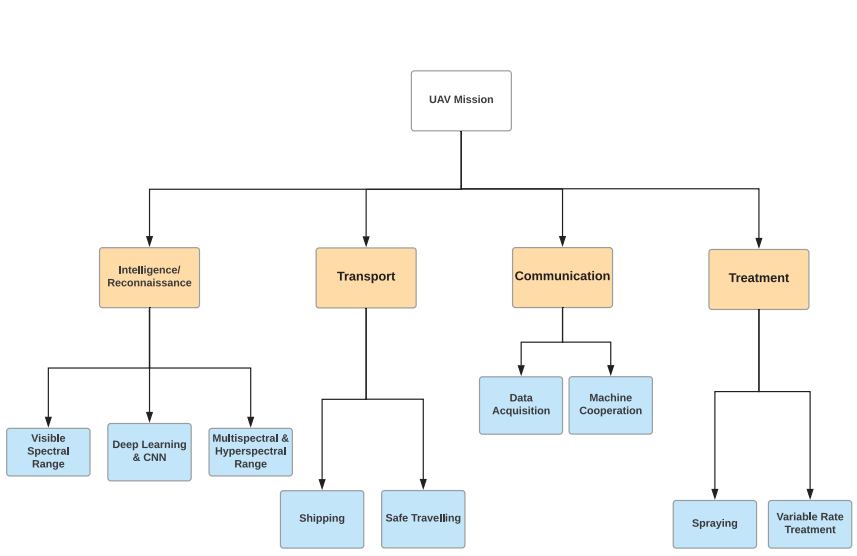
\includegraphics[scale=.5]{Drone_Groups.png}}
\caption{Classification of Drones in PA \cite{Bacco_Smart_2018}}
\label{rein3}
\end{figure}

\bibliography{references}
\chapter{Affidavit}
I, Vytaras Juraska, herewith declare that I have composed the present paper and work by myself and without use of any other than the cited sources and aids. Sentences or parts of sentences quoted literally are marked as such; other references with regard to the statement and scope are indicated by full details of the publications concerned. The paper and work in the same or similar form has not been submitted to any examination body and has not been published. This paper was not yet, even in part, used in another examination or as a course performance.
\end{document}